\chapter{Requirements und Use Cases}\label{ch:requirements-und-use-cases}

\section{Systemebene}\label{sec:systemebene}

%% Die Anforderungen aus der Aufgabenstellung sind nicht vollständig. Die Struktur der nachfolgenden Kapitel soll Sie bei der Strukturierung der Analyse unterstützen. Dokumentieren Sie die Ergebnisse der Analysen entsprechend.

\subsection{Stakeholder}\label{subsec:stakeholder}

%% Ermitteln Sie die Stakeholder für das Projekt und listen Sie diese hier auf.

\paragraph{Externe Stakeholder}
\begin{itemize}
    \item Auftraggeber
    \begin{itemize}
        \item Erfüllung aller spezifizierten Anforderungen
        \item Pünktliche Lieferung zum vorgegebenen Termin
        \item Verwendung der vorgegebenen Hard- und Software
    \end{itemize}
    \item Betreuer
    \begin{itemize}
        \item Erreichen der Ziele am Ende jeder Phase
        \item Möglichst vollständige Dokumentation als Rückmeldungsgrundlage
    \end{itemize}
    \item Benutzer
    \begin{itemize}
        \item System stellt keine Gefahr dar
        \item Information über Fehlerzustände
        \item Möglichst selten Eingreifen erforderlich
        \item Hoher Durchsatz
        \item Einfache Bedienung und Inbetriebnahme (Dokumentation)
    \end{itemize}
    \item Verwaltung TI-Labor
    \begin{itemize}
        \item Keine Beschädigung der Anlagen
    \end{itemize}
\end{itemize}

\paragraph{Interne Stakeholder}
\begin{itemize}
    \item Entwickler
    \begin{itemize}
        \item Gute Testbarkeit
        \item Einfache Erweiterbarkeit und Modularität
        \item Einheitliche Schnittstellen und Benennungen
        \item Dokumentation (im Code) für Fehlersuche und Teamarbeit
    \end{itemize}
\end{itemize}

\subsection{Anforderungen}\label{subsec:anforderungen2}

%! suppress = LabelConvention
\paragraph{\glspl{workpiece} und Sortierung}
\begin{itemize}
    \reqitem{1} Die \gls{anlage} kann zwischen vier Typen von \glspl{workpiece}n unterscheiden (\gls{workpiece_type}) (2, 3, 4, 5, 6)
    \begin{itemize}
        \item \gls{workpiece_flach} (3)
        \item \gls{workpiece_metall} (4)
        \item \gls{workpiece_bohrung} (5)
        \item \gls{workpiece_hoch} (6)
    \end{itemize}
    \reqitem{2} Am Ende des 2.\ \gls{belt}es sollen die \glspl{workpiece} zyklisch in folgender Reihenfolge ankommen (1, 7, 8)
    \begin{enumerate}
        \item \gls{workpiece_metall}
        \item \gls{workpiece_bohrung}
        \item \gls{workpiece_flach}
    \end{enumerate}
    \reqitem{3} \glspl{workpiece}, die nicht in die Sortierreihenfolge passen werden in eine der beiden \glspl{rampe} aussortiert (9, 10)
    \reqitem{4} Der \gls{durchsatz} an \glspl{workpiece} ist zu optimieren (11)
    \reqitem{30} Aussortierung der \glspl{workpiece} soll mit \gls{weiche} funktionieren (41)
    \reqitem{38} Aussortierung der \glspl{workpiece} soll mit \gls{ejector} funktionieren (41)
    \reqitem{39} Beliebige Kombinationen der \gls{sortierer} an den beiden \glspl{anlage} sollen unterstützt werden (42)
    \reqitem{47} Wenn ein \gls{workpiece_bohrung} oder \gls{workpiece_metall} umgedreht wird, ist es ein \gls{workpiece_hoch}
\end{itemize}

\paragraph{Kapazität}
\begin{itemize}
    \reqitem{5} Bei einer vollen \gls{rampe} wird eine Warnung ausgesandt (12)
    \reqitem{6} Wenn die nächste notwendige Aussortierung aufgrund von ausgeschöpfter \glspl{rampe}kapazität
    nicht stattfinden kann, ein Fehler ausgesendet (und somit der Gesamtbetrieb gestoppt) (13)
\end{itemize}

\paragraph{Durchlassablauf}
\begin{itemize}
    \reqitem{7} Zuführung von \glspl{workpiece}n erfolgt durch Einlegen von \glspl{workpiece}n am Anfang von \gls{anlage} 1 (14, 15)
    \begin{itemize}
        \item Ein Unterbrechen der \gls{lb_st} signalisiert dem System das Einlegen eines \gls{workpiece}s,
        sodass der Transport dessen beginnen kann
    \end{itemize}
    \reqitem{9} Das System muss mit in beliebigem Abstand eingelegten \glspl{workpiece}n umgehen können (16, 17) %TODO Mindestabstand
    \begin{itemize}
        \item Solange der Bereich der ersten Lichtschranke frei ist, muss der Benutzer \glspl{workpiece}
        einlegen können, ohne die Korrektheit der Funktion zu gefährden
    \end{itemize}
    \reqitem{14} Der Abstand von \glspl{workpiece}n auf \gls{belt} 2 muss mindestens 25 cm betragen (18)
    \begin{itemize}
        \item Abstand muss vor der Übergabe sichergestellt werden
    \end{itemize}
    \reqitem{16} Auf dem \gls{belt} von \gls{anlage} 2 dürfen sich maximal 2 \glspl{workpiece} befinden (19)
    \reqitem{18} Falls sich bei der Übergabe zwischen den beiden \glspl{belt} ein \glspl{workpiece}
    überschlägt, muss der neue \gls{workpiece_type} beachtet werden (20)
    \begin{itemize}
        \item Der Fall, dass das Teil auf die Seite fällt, sodass es wegrollen könnte, wird ausgeschlossen.
        Wenn sich das \gls{workpiece} überschlägt, ändert sich bei hohen \glspl{workpiece}n der Typ
    \end{itemize}
    \reqitem{20} \glspl{workpiece} dürfen nicht vom \gls{belt} fallen (21)
    \reqitem{24} Beim Einlegen eines \glspl{workpiece}s in die \gls{anlage} soll dem \gls{workpiece} eine eindeutige ID zugewiesen werden(28)
    \reqitem{26} Wenn sich auf einem \gls{belt} kein \gls{workpiece} befindet, stoppt das \gls{belt}
    \reqitem{31} Wenn ein \gls{workpiece} die \gls{lb_en} von FB2 erreicht,
    sollen Informationen zu diesem \gls{workpiece} auf der Konsole ausgegeben werden (22, 23, 24, 25, 26, 27)
    \begin{itemize}
        \item Zu den Informationen zählen die ID, Typ, Höhe auf \gls{anlage} 1 und \gls{anlage} 2 des \gls{workpiece}es als
        auch ein Hinweis darüber, ob sich das \gls{workpiece} überschlagen hat
    \end{itemize}
\end{itemize}

\paragraph{Bedienung durch Taster}
\begin{itemize}
    \reqitem{12} Bei Betätigung von \gls{t_start} wechselt die \gls{anlage} in den Betriebszustand (49)
    \reqitem{15} Bei \gls{longpress} von \gls{t_start} wechselt die \gls{anlage} in den Service-Modus (50)
    \begin{itemize}
        \item Anforderung für den Wechsel ist, dass die \gls{anlage} im Ruhezustand ist
        \item Im Service Modus führt die \gls{anlage} Kalibrierung und Selbsttests durch %TODO Modi in glossar aufnehmen
    \end{itemize}
    \reqitem{17} Bei Betätigung des \gls{t_stop} wechselt die \gls{anlage} in den Ruhezustand (51, 52)
    \begin{itemize}
        \item Wenn Fehler oder Warnung vorliegen, wird stattdessen ein Fehler ausgesandt  %TODO Warnung und Fehler in glossar aufnehmen
    \end{itemize}
    \reqitem{21} Bei Betätigung des \gls{t_reset} werden sämtliche Fehler quittiert (53) %TODO mit kunden kären
    \reqitem{28} Wenn die \gls{anlage} durch \gls{estop} stillgelegt ist, kann der Betrieb durch Drücken des
    \gls{t_reset} der \gls{anlage}, an dem auch der \gls{estop} gedrückt wurde, fortgesetzt werden (56) %TODO 'fortsetzten' mit kunden kären
    \begin{itemize}
        \item Bedingung dafür: Keine \gls{estop} sind gedrückt
    \end{itemize}
    \reqitem{40} Im Service Modus führt die \gls{anlage} Kalibrierung und Selbsttests durch (50) %TODO genauer spezifizieren
    \reqitem{41} Bei Betätigung eines \gls{estop} werden beide \glspl{anlage} angehalten (54, 55)
    \reqitem{42} Dem Benutzer werden Hinweise über die Benutzung der \gls{anlage} mithilfe der LEDs an der \gls{taster}n gegeben
    \begin{itemize}
        \item Im Betriebszustand ist die LED am \gls{t_start} an
        \item Im Ruhezustand die LED am \gls{t_stop}
        \item Bei einem gegangenen oder bestehenden Fehler ist die LED am \gls{t_reset} an
    \end{itemize}
\end{itemize}

\paragraph{Zustandsanzeigen}
\begin{itemize}
    \reqitem{10} Im Betriebszustand leuchtet die grüne \gls{ampelled} dauerhaft (59)
    \reqitem{11} Im Service-Mode blinkt die grüne \gls{ampelled}  (60)
    \reqitem{13} Bei Warnungen blinkt die gelbe \gls{ampelled} (61)
    \begin{itemize}
        \item Eine Warnung ist, dass die \gls{rampe} an der \gls{anlage} voll ist
    \end{itemize}
    \reqitem{19} Wenn im Betriebszustand keine Warnungen vorliegen, ist die gelbe \gls{ampelled} aus (61)
    \reqitem{37} Die rote \gls{ampelled} signalisiert die Fehlerzustände wie folgt (73, 74, 75, 76):
    \begin{itemize}
        \item Anstehend unquittiert wird durch schnelles Blinken (1 Hz) signalisiert (74)
        \item Anstehend quittiert wird durch dauerhaftes Leuchten(75) signalisiert
        \item Gegangen unquittiert wird durch langsames Blinken (0,5 Hz) signalisiert (z.B.\ wenn ein
        \gls{workpiece} an einer \gls{weiche} zu langsam in die \gls{rampe} geschoben wurde) (76)
        \item Steht kein Fehler an, ist die Leuchte aus (73)
    \end{itemize}
    \reqitem{45} Im Ruhezustand leuchtet die \gls{ampel} dauerhaft gelb
\end{itemize}

\paragraph{\gls{weiche}}
\begin{itemize}
    \reqitem{23} Bei Verklemmen der \gls{weiche} wird eine Warnung ausgesandt, bis das \gls{workpiece} in der Rampe ankommt (37)
    \begin{itemize}
        \item Ein \gls{workpiece} ist verklemmt, wenn das \gls{workpiece} länger als erwartet braucht, um in der \gls{rampe} anzukommen
        \item Länger als erwartet wird mit mehr als 50 Prozent der durchschnittlichen Aussortierzeit definiert
    \end{itemize}
    \reqitem{27} Die \gls{weiche} darf nicht länger als 'x' auf offen stehen (35, 36) %TODO 'offen' , zeit festlegen
    \begin{itemize}
        \item Bei minutenlangen Stromfluss wird die \gls{weiche} beschädigt
    \end{itemize}
\end{itemize}

\paragraph{\gls{recorder}}
\begin{itemize}
    \reqitem{25} Es soll eine \gls{record-fn} bereitgestellt werden, mit der ein Benutzer alle
    \glspl{event} der \gls{anlage} in ein \gls{protokoll} aufzeichnen kann (90)
    \reqitem{29} Die von der \gls{record-fn} vorgenommene Aufzeichnung soll menschenlesbar sein (91)
    \reqitem{33} Es soll eine \gls{replay-fn} bereitgestellt werden, mit der ein
    Benutzer eine zuvor aufgezeichnetes \gls{protokoll} abspielen lassen kann (93, 94)
    \reqitem{34} \glspl{protokoll} sollen per Hand angefertigt werden können (95, 96)
\end{itemize}

\paragraph{Höhenmessung}
\begin{itemize}
    \reqitem{32} Bei der Auswertung der Höhenmessung ist die durch Verkippung des Sensors entstehende Abweichung zu berücksichtigen (43, 44)
\end{itemize}

\paragraph{Fehlerumgang}
\begin{itemize}
    \reqitem{35} Nach Behebung eines Fehlers soll der Normalbetrieb fortgesetzt werden (45, 46)
    \begin{itemize}
        \item Nach Möglichkeit sollen die \glspl{belt} nicht geräumt werden
    \end{itemize}
    \reqitem{43} In den Zuständen 'bestehend\_unquittiert' und 'bestehend\_quittiert' bleiben die
    \glspl{belt} beider \glspl{anlage} stehen und der \gls{sortierer} wird der Strom abgestellt
    \begin{itemize}
        \item Die Fehleranzeige mittels der \gls{ampel} ist in\refreq{37}spezifiziert
    \end{itemize}
    \reqitem{36} Fehlerzustand soll wie in Abbildung~\ref{fig:stm-fehlerzustand} beschrieben sein. (65, 66, 67, 69, 70)
    \reqitem{46} Der Fehlerzustand beider \glspl{anlage} wird wie folgt festgelegt:
    \begin{itemize}
        \item Der aktuell bestehende Fehler mit der höchsten Priorität entspricht dem Fehlerzustand der gesamten \gls{anlage}.
        Die Fehlerzustände sind der folgenden Liste nach priorisiert:
    \begin{enumerate} %TODO wording anpassen sodass kein 'priorität' vorkommnt
        \item Anstehend unquittiert
        \item Anstehend quittiert
        \item Gegangen unquittiert
        \item OK
    \end{enumerate}
    \end{itemize}
\end{itemize}

\begin{figure}[h]
    \centering
    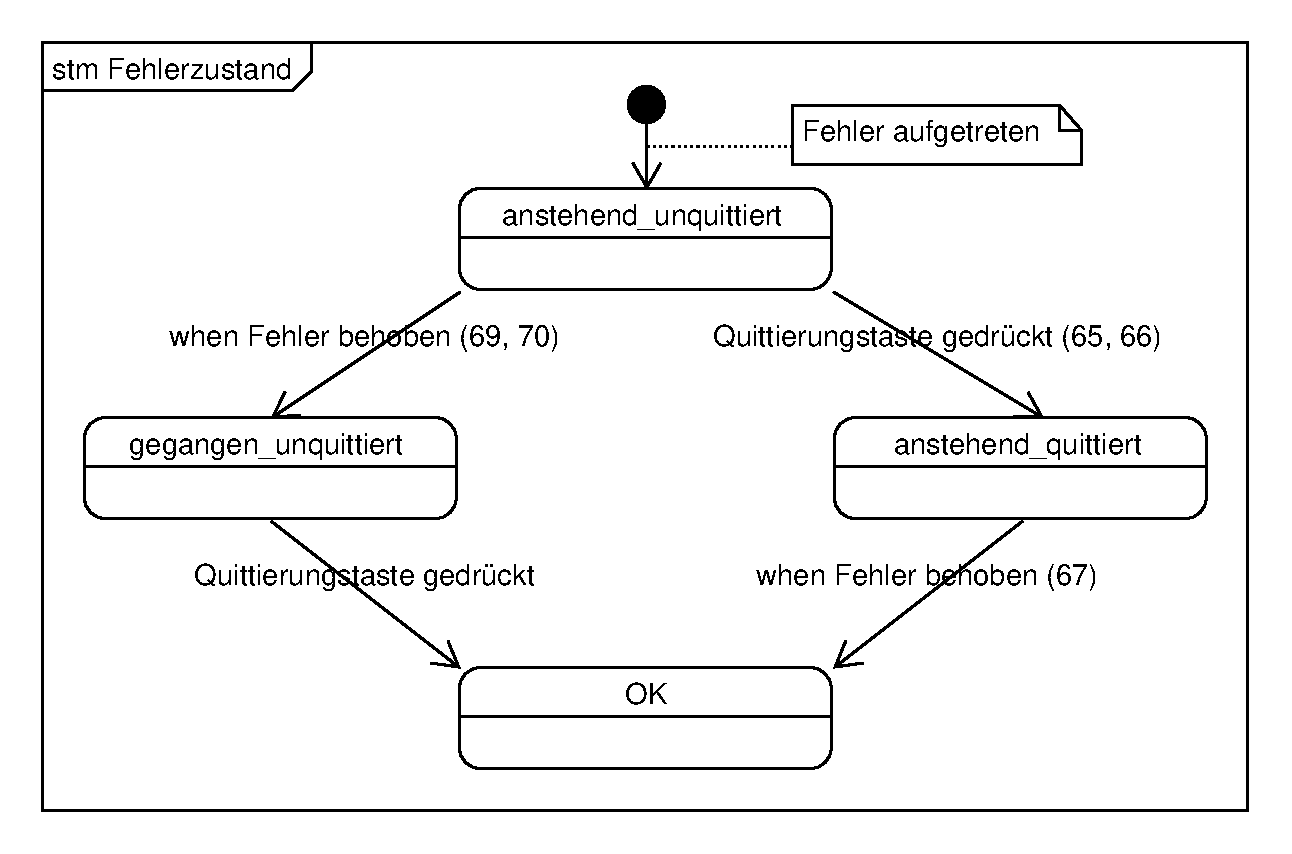
\includegraphics[scale=0.5]{../out/diagrams/stage1/req-fehlerzustand}
    \caption{REQ-36 Visualisierung des Fehlerzustandes eines einzelnen Fehlers}
    \label{fig:stm-fehlerzustand}
\end{figure}

\FloatBarrier

%% In der Aufgabenstellung sind Anforderungen an das System gestellt.
%% Arbeiten Sie diese hier auf und ergänzen Sie diese entsprechend der Absprachen mit dem Betreuer.
%% Achten Sie auf die entsprechende Atribuierung.
%% Berücksichtigen Sie auch mögliche Fehlbedienungen und Fehlverhalten des Systems.

\subsection{Systemkontext}\label{subsec:systemkontext2}

\begin{figure}
    \centering
    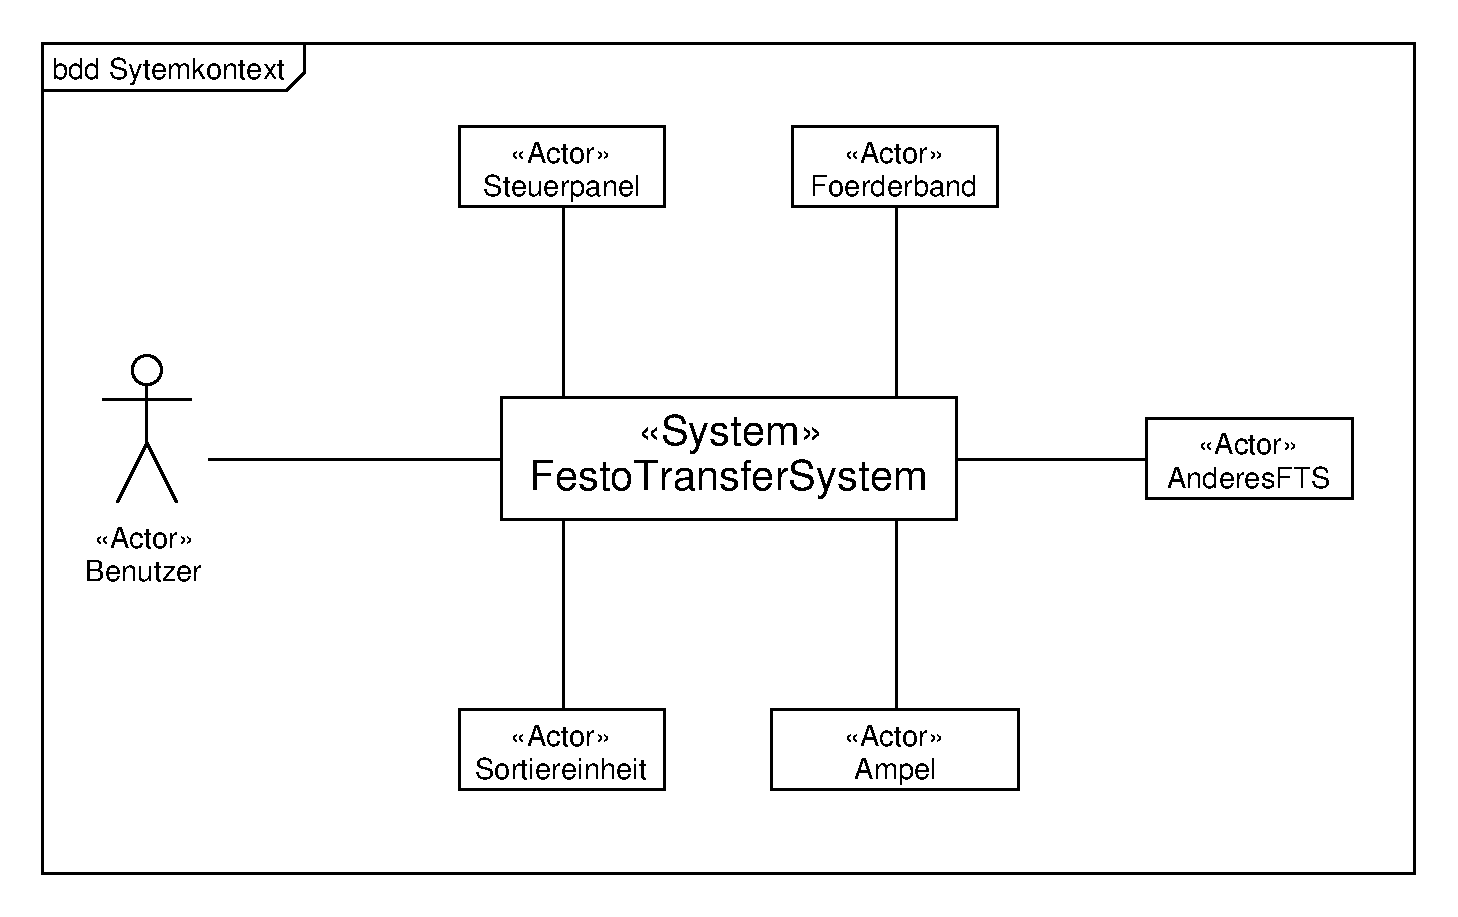
\includegraphics[width=\textwidth]{../out/diagrams/stage1/systemkontext.pdf}
    \caption{Systemkontext}
    \label{fig:systemkontext}
\end{figure}


Betrachte Abbildung \ref{fig:systemkontext}.
Die Systemsicht bringt umliegende Aktorik des Systemkontext und System selber miteinander in Beziehung.

\paragraph{Akteure}

\begin{itemize}
    \item Control\_Panel\\
    Steuerungspanel der Anlage.
    Sie stellt einen START-, STOP- und RESET-Button zur Verfügung.

    \item Conveyor\_Belt\\
    Auf Förderband werden Werkstücke durch das System bewegt.
    \item FTS\_2\\
    Die jeweils andere Förderanlage, mit der das System kommuniziert.
    \item E\_Stop\\
    Ein Button zum Auslösen des Emergency-Stops.
    \item Metal\_Detector\\
    Metall-Sensor zum Erfassen des Materials eines Werkstückes.
    \item Height\_Measurement\\
    Höhen-Sensor zum Erfassen des Materials eines Werkstückes.
    \item Stoplight\\
    Ampel, die durch verschiedene LED-Einstellungen Zustandsinformationen der Anlage anzeigt.
    \item Sorting\_Mechanism\\
    Das System besitzt allgemein einen Aussortier-Mechanismus.
    Dieser ist in einer von zwei Varianten in die Anlage eingebaut:
    \begin{itemize}
        \item Ejector\\
        Ein Auswerfer, der sich bei Stromzufluss ausfährt und so Werkstücke in die Rampe stoßen soll.
        Ohne Strom ist der Aussortiermechanismus offen.
        \item Switch\\
        Eine Weiche, die sich bei Stromzufluss öffnet und Werkstücke durchlässt.
        Ohne Strom ist der Aussortiermechanismus geschlossen und befördert Werkstücke langsam in die Rampe.
    \end{itemize}
    \item LightBarrier\\
    Das System besitzt diverse Lichtschranken als Trigger und zur Steuerung des Kontrollflusses
    \begin{itemize}
        \item LightBarrier\_Start\\
        Lichtschranke am Anfang eines Förderbandes.
        Die Unterbrechung dieser Lichtschranke setzt das Förderband in Bewegung.
        \item LightBarrier\_Ramp\\
        Lichtschranke an der Rampe, in der die Werkstücke aussortiert werden.
        Die kurze Unterbrechung dieser Lichtschranke kann als erfolgreiche Aussortierung interpretiert werden.
        Eine stetige Unterbrechung signalisiert eine volle Rutsche.
        \item LightBarrier\_Height\\
        Lichtschranke an der Position des Höhensensors.
        Die Unterbrechung dieser Lichtschranke startet eine Höhenmessung.
        \item LightBarrier\_Switch\\
        Lichtschranke vor dem Aussortiermechanismus der Anlage.
        Die Unterbrechung startet den Aussortieralgorithmus.
        \item LightBarrier\_End\\
        Lichtschranke am Ende eines Förderbandes.
        Die Unterbrechung dieser Lichtschranke kann das transferieren des Werkstückes an die nächste Anlage einleiten.
        Am Ende der zweiten Anlage werden bei Unterbrechung dieser Lichtschranke Werkstück-Informationen an der Konsole ausgegeben.
    \end{itemize}
\end{itemize}

%% Use Cases werden aus einer bestimmten Sicht erstellt.
%% Dokumentieren Sie diese mittels Kontextdiagramm oder Use Case Diagramm.
%% Die Use Cases und Test Cases müssen zu der hier verwendeten Nomenklatur konsistent sein.

\subsection{Use Cases / User Stories}\label{subsec:use-cases-user-stories}

%% Dokumentieren Sie hier, welche Use Cases/ User Stories Sie auf der Systemebene implementieren müssen.
%% Die Test Cases sollen später zu den Use Cases/ User Stories konsistent sein.

%% < Hier kommt die genaue Beschreibung der Use.
%% Pro Anforderung eine Tabelle benutzen. Die Tabelle nach Belieben vervielfältigen. >

\begin{usecase}{1}{UseCase Name}{hoch}
\addCollum{Mainflow}{
\item[1)] do something
\item[2)] do this
\item[2a)] or tihs
}\addCollum{Alternate flow}{
\item[1)] do something
\item[2)] do this
\begin{itemize}
    \item[1)] Very long text: Lorem ipsum dolor sit amet, consectetur adipiscing elit,
    \item[2)] do this
\end{itemize}
\item[2a)] or tihs
}
\end{usecase}
\addTextCollum{Description}{
    Lorem ipsum dolor sit amet, consectetur adipiscing elit,
    sed do eiusmod tempor incididunt ut labore et dolore magna aliqua.
    Ut enim ad minim veniam, quis nostrud exercitation ullamco laboris
    nisi ut aliquip ex ea commodo consequat. Duis aute irure dolor in
    reprehenderit in voluptate velit esse cillum dolore eu fugiat nulla pariatur.
    Excepteur sint occaecat cupidatat non proident, sunt in culpa qui officia
    deserunt mollit anim id est laborum
}

\begin{usecase}{03}{Handle Lightbarrier\_Switch}{hoch}
    \addTextCollum{Description}{
        Bindeglied zwischen \nameref{uc:02}, \nameref{uc:06} und \nameref{uc:15},
    }
    \addTextCollum{Trigger}{
        Light\_Barrier\_Switch unterbrochen
    }
    \addCollum{Mainflow}{
        \item[1)] UC2 determine sorting action
        \item[2)] Sorting action ist \gls{discard} \textbullet
        \item[3)] UC6 \gls{discard}
    }
    \addCollum{Alternate flow}{
        \item at step 2) of Mainflow
        \item[2a)] Sorting action ist \gls{do_not_discard}\_workpiece
        \begin{itemize}
            \item[2a1)] UC15 \gls{do_not_discard}\_workpiece
            \item[2a1)] Ende des use cases
        \end{itemize}
    }
    % postconditions sind in den jeweiligen unter UCs gehandelt.
\end{usecase}

% eine referenz zu einem UC sieht so aus:
siehe  \nameref{uc:1}.

\begin{usecase}{06}{Discard workpiece}{hoch}
    \addTextCollum{Verwandte Requirements}{
        REQ-3, REQ-5, REQ-23, REQ-30, REQ-38, REQ-39
    }
    \addTextCollum{Description}{
    In diesem Use-Case bewegt der Aussortiertmechanismus der Anlage ein Werkstück vom Förderband in die Rutsche
    }
    \addTextCollum{Actors}{
    LightBarrier\_Switch, LightBarrier\_Ramp, SortingMechanism
    }
    \addCollum{Precondition}{
    \item Anlage befindet sich im Betriebszustand
    \item Dass das betroffene Werkstück aussortiert werden soll ist festgelegt
    }
    \addCollum{Trigger}{
    \item LightBarrier\_Switch unterbrochen
    }
    \addCollum{Mainflow}{
    \item[1)] Führe Aussortierung durch
    \item[2)] Warte auf Unterbrechung von LightBarrier\_Ramp
    \item[3)] LightBarrier\_Ramp wurde ausgelöst
    }

    \addCollum{Postcondition}{
    \item Werkstück liegt in der Rampe
    \item LightBarrier\_Switch nicht mehr unterbrochen
    }


    \addCollum{Exceptional flow 1}{
        \item at step 3) of Mainflow
        \item[1)] LightBarrier\_Ramp ist nach der 1,5-fachen durchschnittlichen Aussortierzeit nicht ausgelöst worden
        \item[2)] Warnung wird gesendet
    }
    \addCollum{Postcondition of e.f.}{
        \item LightBarrier\_Switch nicht mehr unterbrochen
        \item Eine Warnung über das Feststecken des Werkstückes liegt vor
    }
\end{usecase}


\begin{usecase}{12}{Handle Error}{hoch}
    \addTextCollum{Verwandte Requirements}{
        REQ-21, REQ-36, REQ-37, REQ-43, REQ-46
    }
    \addTextCollum{Actors}{
        Stoplight, Control\_Panel
    }
    \addTextCollum{Description}{
        Der ErrorHandler verwaltet alle Fehler, die im System auftreten. Immer wenn ein Fehler-Event ausgelöst wird,
        legt der ErrorHandler diese in eine Fehlerliste ab. Jeder Fehler hat einen Fehlerzustand,
        welcher wie in der Statemachine~\ref{fig:stm_fehler} beschrieben ist.
        Wenn der Reset-Taster gedrückt wird, werden alle Fehler in der Fehlerliste quittiert.
        Fehler gelten als behoben, wenn ein Event die Behebung des Fehlers meldet.
        Der Fehlerzustand der gesamten Anlage, somit auch die Anzeige der roten LED,
        wird durch den dem Fehler mit der höchsten Priorität in der Fehlerliste festgelegt. Die Fehlerzustände sind wie in Fehlerpriorität priorisiert.
        Ist der globale Fehlerzustand anstehend\_unquittiert oder anstehend\_quittiert,
        dann bleiben die Laufbänder beider Anlagen stehen und der Strom an den Aussortiermechanismen wird abgestellt.
    }
    \addCollum{Fehlerpriorität}{
        \item[1)] anstehend\_unquittiert. Wird durch ein dauerhaftes leuchten der roten LED signalisiert.
        \item[2)] anstehend\_quittiert. Wird durch wird durch schnelles Blinken (1 Hz) der roten LED signalisiert.
        \item[3)] gegangen\_quittiert . Wird durch wird durch langsames Blinken (0,5 Hz) der roten LED signalisiert.
    }
\end{usecase}

\begin{usecase}{07}{E-Stop}{hoch}
    \addCollum{Verwandte Requirements}{
    \item REQ-41, REQ-42, REQ-28,
    }
    \addTextCollum{Description}{
        Dieser Use-Case beschreibt den Umgang des Systems bei Betätigung des E-Stop-Schalters.
    }
    \addCollum{Actors}{
    \item E\_Stop, FTS\_2, Stoplight, Control\_Panel, Sorting\_Mechanism, Conveyor\_Belt
    }
    \addCollum{Precondition}{}
    \addCollum{Triggers}{
        \item[1a)] E\_Stop-Taster von FTS wird betätigt
        \item[1b)] E\_Stop-Schalter von FTS\_2 wird betätigt
    }
    \addCollum{Mainflow}{
        \item[1)] Der aktuelle Zustand sämtlicher Sensoren und Aktoren von FTS und FTS\_2 wird gespeichert
        \item[2)] Conveyor\_Belt, Sorting\_Mechanism von FTS und FTS\_2 werden abgeschaltet.
        \item[3)] Die Lampe am FTS und FTS\_2 leuchtet dauerhaft rot.
        \item[4)] E\_Stop-Schalter von FTS wird herausgezogen
        \item[5)] Reset-Taster von FTS wird gedrückt
    }
    \addCollum{Alternate flow}{
        \item at step 4) of Mainflow
        \item[2a)] E\_Stop-Schalter von FTS\_2 wurde betätigt
        \begin{itemize}
            \item[2a)] E\_Stop-Schalter von FTS\_2 wird herausgezogen
            \item[2b)] Reset-Taster von FTS\_2 wird gedrückt
        \end{itemize}
    }
    \addCollum{Postcondition}{
    \item Das System befindet sich im Ruhezustand.
    }
\end{usecase}

%! Author = justi
%! Date = 23.04.2021

% Preamble
\documentclass[11pt]{article}

% Packages
\usepackage{amsmath}

% Document
\begin{document}



\end{document}

\begin{usecase}{11}{Run Service}{hoch}
    \addTextCollum{Verwandte Requirements}{
        REQ-11, REQ-15, REQ-40
    }
    \addTextCollum{Description}{
        Dieser Usecase betreibt das Durchführen des Servicemode. 
        Dieser kann durch das lange drücken des Starttasters von beiden Anlagen aus aktiviert werden.
        Im Servicemode werden die Höhenmesser kalibriert sowie die korrekte Funktion des Aussortiermechanismus geprüft
    }
    \addCollum{Actors}{
        \item Stoplight
        \item Height\_Measurement
        \item Control\_Panel
        \item Sorting\_Mechanism
    }
    \addCollum{Preconditions}{
        \item System ist im Ruhezustand
    }
    \addCollum{Triggers}{
        \item Start-taster wird lange gedrückt
        \item Mitteilung von FTS\_2 über Betreten des Service
    }
    \addCollum{Mainflow}{
        \item[1)] Mitteilung an FTS\_2 über Betreten des Service senden
        \item[2)] Stoplight grün blinken lassen
        \item[3)] Messung bei Height\_Measurement anfragen
        \item[4)] Auf Rückmeldung warten
        \item[5)] Bestimmten Wert als Nullwert im Height\_Measurement eintragen
        \item[6)] Sorting Mechanism aktivieren
        \item[7)] Auf Zustandsänderungssignal des Sorting\_Mechanism warten \textbullet
        \item[8)] Sorting Mechanism deaktivieren
        \item[9)] Auf Zustandsänderungssignal des Sorting\_Mechanism warten \textbullet
        \item[10)] In Betriebszustand wechseln
    }
    \addCollum{Postconditions}{
        \item[1)] System ist im Ruhezustand
        \item[2)] Height\_Measurement wurde kalibriert
    }
    \addCollum{Exceptional flow 1}{
        \item at step 6 or 8 of Mainflow
        \item[1)] Timeout beim Empfang des Signals
        \item[2)] Fehler auslösen
    }
    \addCollum{Postconditions of Exceptional Flow 1}{
        \item[1)] System ist im Fehlerzustand
    }
\end{usecase}


\begin{usecase}{04}{Transfer Workpiece}{mittel}
    \addTextCollum{Verwandte Requirements}{
    REQ-9, REQ-14, REQ-16, REQ-18, REQ-31
    }
    \addTextCollum{Description}{
    In diesem Use-Case erreicht ein Werkstück das Ende eines Förderbandes und wird gegebenenfalls an das nächste Förderband transferiert
    }
    \addTextCollum{Actors}{
    Conveyor\_Belt, FTS\_2, LightBarrier\_End
    }

    \addCollum{Precondition}{
    \item Anlage befindet sich im Betriebszustand
    }

    \addCollum{Trigger}{
    \item LightBarrier\_End wird unterbrochen
    }

    \addCollum{Mainflow}{
    \item[1)] Die Anlage ist in Primary Mode \textbullet
    \item[2)] Conveyor\_Belt stoppen
    \item[3)] Anfrage zum transferieren und Werkstück\-Informationen an FTS\_2 senden
    \item[4)] Auf 'OK' von FTS\_2 warten
    \item[5)] Conveyor\_Belt in Bewegung setzen und Werkstück transferieren
    }

    \addCollum{Alternative Flow 1}{
    \item at step 1) of Mainflow
    \item[1a)] Die Anlage ist in Secondary Mode
    \begin{itemize}
        \item[1a1)] Ausgabe der ID, des Typs, Höhe\_FB1 und Höhe\_FB2 auf der Konsole
        \item[1a2)] Ausgabe an der Konsole, ob sich das Werkstück bei der Übergabe zwischen den Anlagen überschlagen hat
    \end{itemize}
    }

    \addCollum{Postcondition}{
    \item Werkstück ist nicht mehr auf dem Förderband
    }
\end{usecase}

\begin{usecase}{9}{Start System}{hoch}
    \addTextCollum{Verwandte Requirements}{
        REQ-12, REQ-42
    }
    \addCollum{Actors}{
        \item FTS\_2
        \item Control\_Panel
    }
    \addCollum{Preconditions}{
        \item System ist gestoppt
        \item System ist nicht im Fehlerzustand
    }
    \addCollum{Trigger}{
        \item Der Startknopf auf dem Steuerpanel wird gedrückt
        \item FTS\_2 schickt signal zum Starten
    }
    \addCollum{Mainflow}{
        \item[1)] System wechselt in den Betriebszustand \textbullet
        \item[2)] LED im Stopptaster wird ausgeschaltet
        \item[3)] LED im Starttaster wird eingeschaltet \textbullet
    }
    \addCollum{Alternate flow 1}{
        \item at step 1 of Mainflow
        \item[1)] Trigger ist Drücken des Knopfes
        \item[2)] Signal zum Starten an FTS\_2 schicken
        \item[3)] Auf Bestätigung von FTS\_2 warten \textbullet
        \item[4)] mit Mainflow Step 1 weitermachen
    }
    \addCollum{Alternate flow 2}{
        \item at step 3 of Mainflow
        \item[1)] Trigger ist Signal von FTS\_2 des Knopfes
        \item[2)] Signal Bestätigung an FTS\_2 schicken
    }
    \addCollum{Postconditions}{
        \item[2)] FTS\_2 ist im Betriebszustand
        \item[3)] System ist im Betriebszustand
    }
    \addCollum{Exceptional flow 1}{
        \item at step 3 of Alternate Flow 1
        \item[1)] Timeout
        \item[2)] In Fehlerzustand wechseln
    }
\end{usecase}


\begin{usecase}{16}{Answer Transfer Request}{mittel}
    \addTextCollum{Verwandte Requirements}{
    REQ-9, REQ-14, REQ-16, REQ-18, REQ-31
    }
    \addTextCollum{Description}{
    In diesem Use-Case wird eine Transfer Request, die von der Master-Anlage ausgeht, von der Slave-Anlage beantwortet
    }
    \addTextCollum{Actors}{
    Conveyor\_Belt, FTS\_2, LightBarrier\_Height, LightBarrier\_Start
    }
    \addCollum{Precondition}{
    \item Anlage ist im Betriebszustand
    \item Anlage befindet sich im Secondary Mode
    }
    \addCollum{Trigger}{
    \item Transfer Request mit Workpiece-Info von FTS\_2
    }
    \addCollum{Mainflow}{
    \item[1)] Kein Werkstück befindet sich zwischen LightBarrier\_Start und LightBarrier\_Height \textbullet
    \item[2)] Sende 'OK' an FTS\_2
    }

    \addCollum{Alternative Flow 1}{
    \item at stept 1) of Mainflow
    \item[1a)] Es befindet sich ein Werkstück zwischen LightBarrier\_Start und LightBarrier\_Height
    \begin{itemize}
        \item[1a1)] Warten auf Unterbrechung von LightBarrier\_Height
        \item[1a1)] Go back to step 2) of Mainflow
    \end{itemize}
    }

    \addCollum{Postcondition}{
    \item Transfer Request beantwortet
    }
\end{usecase}

\begin{usecase}{02}{Determine Sorting Action}{hoch}
    \addCollum{Precondition}{
        \item Dem workpiece ist ein workpiece\_type zugeordnet
    }
    \addCollum{Actors}{
        \item LightBarrier\_Ramp
    }
    \addTextCollum{Description}{
        Es wird bestimmt, ob ein workpiece aussortiert werden soll, oder nicht.
        Dafür muss der Vorgänger workpiece\_type gespeichert werden.
    }
    \addCollum{Main flow}{
        \item[1)] Der aktuelle workpiece\_type wird mit dem erwarteten verglichen
        \item[2)] Das workpiece stimmt nicht überein, das workpiece muss aussortiert werden \textbullet
        \item[3)] Das workpiece wird mit discard markiert \textbullet
    }
    \addCollum{Alternative flow 1}{
        \item at step 2 of main flow
        \item[2a)] Das workpiece stimmt überein
        \begin{itemize}
            \item[2a1)] Das workpiece wird mit do\_not\_discard markiert
            \item[2a2)] Ende des use case
        \end{itemize}
    }
    \addCollum{Alternative flow 2}{
        \item at step 3 of main flow
        \item[3a)] Rutsche ist voll und in Primary mode
        \begin{itemize}
            \item[3a1)] das Teil mit do\_not\_discard markiert
        \end{itemize}
        \item[3b)] Rutsche ist voll und in Secondary mode
        \begin{itemize}
            \item[3b1)] Gesamtbetrieb wird gestoppt (REQ-6)
        \end{itemize}
    }    
    \addTextCollum{Postcondition}{
        Dem workpiece ist entweder do\_not\_discard oder discard zugeordnet
    }
    \addTextCollum{Verwandte Requirements}{
        REQ-1, REQ-2, REQ-3, REQ-6
    }
\end{usecase}


\begin{usecase}{10}{UseCase Bootup Configuration}{hoch}
    \addCollum{Actors}{
        \item[] FTS_2
        \item[] Control_Panel
    }
    \addCollum{Preconditions}{
        \item[] System ist mit Strom versorgt und Hochgefahren
    }
    \addCollum{Mainflow}{
        \item[1)] HAL wird initialisiert
        \item[2)] Herstellen einer Verbindung zu FTS_2
        \item[3)] Kontrolleuchte 1 auf Control_Panel Blink_Slow aktivieren
        \item[4)] Warten auf Drücken des Startknopfes auf dem ControlPanel
        \item[5)] EVNT_SW_COMM_PRI_REQ an FTS_2 schicken
        \item[6)] Warten auf EVNT_SW_COMM_SEC_AKC von FTS_2
        \item[7)] Eigenen Betriebsmodus auf PRIMARY setzen
        \item[8)] EVNT_SW_COMM_PRI_AKC an FTS_2 schicken
        \item[9)] Kontrolleuchte 1 auf Control_Panel dauerhaft aktivieren
    }
    \addCollum{Alternate flow 1}{
        \item[] at step 4 of Mainflow
        \item[1)] Event EVNT_SW_COMM_PRI_REQ von FTS_2 Empfangen
        \item[2)] Eigenen Betriebsmodus auf SECONDARY setzen
        \item[3)] EVNT_SW_COMM_SEC_AKC an FTS_2 senden
        \item[4)] auf EVNT_SW_COMM_PRI_AKC von FTS_2 warten
        \item[5)] Eigenen Betriebsmodus auf SECONDARY setzen
        \item[6)] Kontrolleuchte 1 auf Control_Panel dauerhaft aktivieren 
    }
    \addCollum{Alternate flow 2}{
        \item[] at step 2 of Mainflow
        \item[1)] Verbindung schlägt fehl
        \item[3)] Zurück in Schritt 2 Mainflow 
    }
    \addCollum{Postconditions}{
        \item[1)] HAL ist initialisiert
        \item[2)] Verbindung mit FTS_2 hergestellt
        \item[3)] Betriebsmodus der Anlage ist festgelegt
    }
    \addCollum{Exceptional flow 1}{
        \item[] at step 1 of Mainflow
        \item[1)] Initialisierung der HAL schlägt fehl
        \item[2)] Fehlermeldung ausgeben
        \item[3)] System abschalten
    }
    \addCollum{Exceptional flow 2}{
        \item[] at step 6 of Mainflow
        \item[1)] Timeout beim Empfangen von EVNT_SW_COMM_SEC_AKC
        \item[2)] Fehler COMM_ERROR auslösen
    }
    \addCollum{Exceptional flow 3}{
        \item[] at step 4 of Alternate flow
        \item[1)] Timeout beim Empfangen von auf EVNT_SW_COMM_PRI_AKC
        \item[2)] Fehler COMM_ERROR auslösen
    }
\addTextCollum{Description}{
    Dieser Use Case beschreibt die Initialisierung des Systems, sowie die Bestimmung von Primary und Secondary-Anlage.
    Das Primary System wird bestimmt
    Verwendete Signale sind EVNT_SW_COMM_PRI_REQ (Sendendes System will Primary sein), 
    EVNT_SW_COMM_SEC_AKC (Acknoledgement vom Secondary nach Empfang) und EVNT_SW_COMM_PRI_AKC (Abschließender Handshake)
}
\end{usecase}

\begin{usecase}{17}{Detect Material}{hoch}
    \addTextCollum{Verwandte Requirements}{
        REQ-1, REQ-2, REQ-3
    }
    \addTextCollum{Description}{
        In diesem Use-Case wird das Material eines Werkstückes erfasst.
        Grundsätzlich wird angenommen, dass ein Werkstück aus Kunststoff ist.
    }
    \addTextCollum{Actors}{
        Metal\_Detector
    }
    \addCollum{Precondition}{
        \item Die Anlage befindet sich im Betriebszustand
    }
    \addCollum{Trigger}{
        \item Metal\_Detector erfasst Metall
    }
    \addCollum{Mainflow}{
        \item[1)] Aktuellem Werkstück wird 'Metall' als Material zugewiesen
    }
    \addCollum{Postcondition}{
        \item Werkstück wurde Material 'Metall' zugewiesen
    }
\end{usecase}

\begin{usecase}{14}{Measure Height}{hoch}
    \addTextCollum{Description}{
        Die Höhe eines workpieces wird gemessen und das Höhenprofil dessen bestimmt.
    }
    \addTextCollum{Actors}{
        Height\_Measurement
    }
    \addTextCollum{Trigger}{
        LightBarrier\_Height
    }
    \addCollum{Mainflow}{
        \item[1)] Messung bei Height\_Measurement anfragen
        \item[2)] Auf Rückmeldung warten
        \item[3)] Rückgabewert mit den in Höhenprofile erwähnten Werten vergleichen
        \item[4)] Rückgabewert fällt in einen der Bereiche (plus Toleranz) \textbullet
        \item[4)] Jeweiliges Höhenprofile zurückgeben
    }
    \addCollum{Exceptional Flow}{
        \item at item 4) of main flow
        \item[4)] Rückgabewert liegt außerhalb aller Bereiche
        \begin{itemize}
            \item Fehlermeldung ausgeben
        \end{itemize}
    }
    \addCollum{Additional Information}{
        \item Höhenprofile
        \begin{itemize}
            \item BOHRUNG 15,8 bis 16,4mm
            \item FLACH 21,0mm
            \item HOCH 25,0 bis 25,4mm
        \end{itemize}
    }
\end{usecase}


\begin{figure}
    \centering
    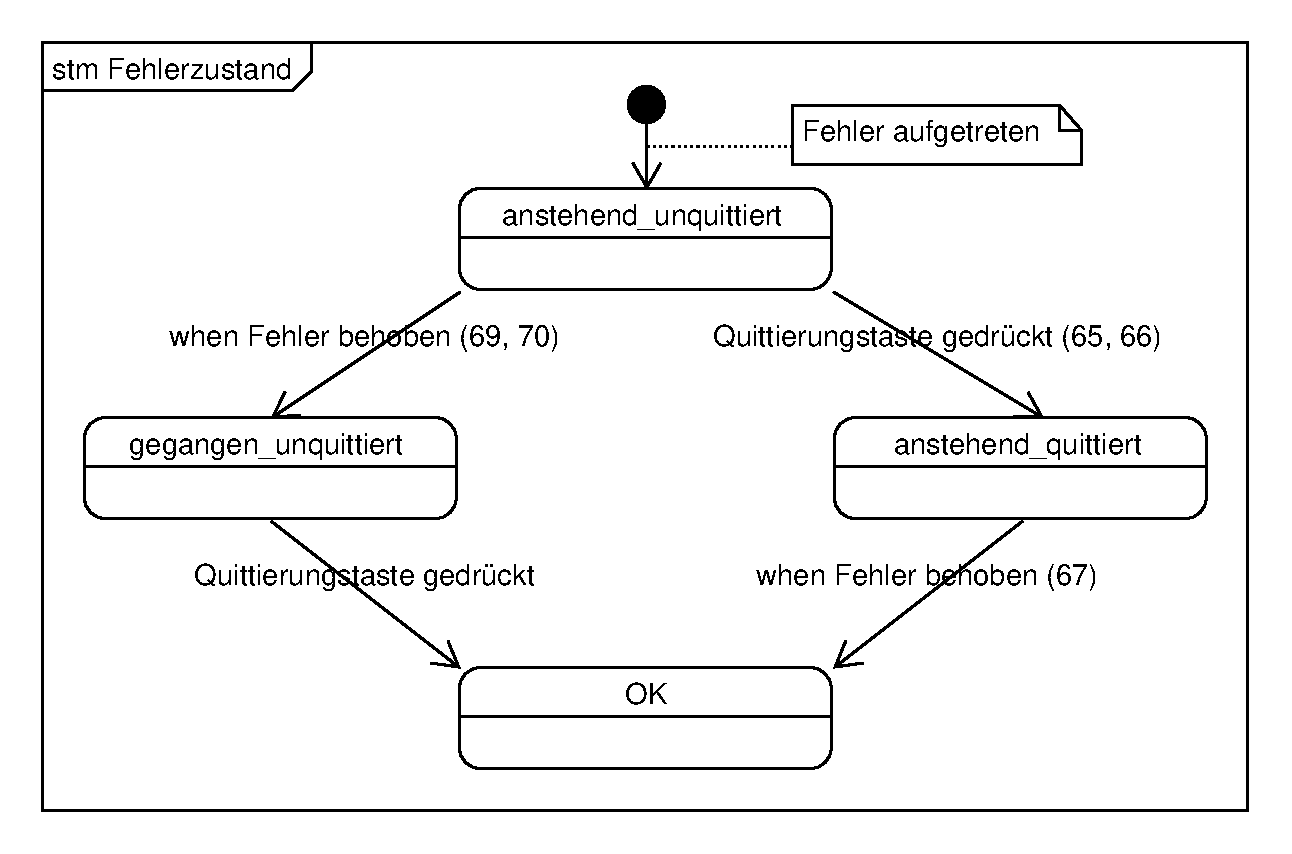
\includegraphics[width=\textwidth]{../out/diagrams/stage1/req-fehlerzustand.pdf}
    \caption{Fehlerzustände}
    \label{fig:stm_fehler}
\end{figure}


\section{Systemanalyse}\label{sec:systemanalyse}

%% Ihr technisches System hat aus Sicht der Software bestimmte Eigenschaften.
%% Was muss man für die Entwicklung der Software in Struktur, Schnittstellen,
%% Verhalten und an Besonderheiten wissen?
%% Wählen Sie eine Kapitelstruktur, die am besten zur Dokumentation Ihrer Ergebnisse geeignet ist.

\subsection{Art des Systems}

Bei dem zu entwerfenden System handelt es sich um die Steuerung eines Festo-Transfersystems, welche auf einem in die Anlage integrierten BeagleBoneBlack Einplatinencomputer zu realisieren ist.
Daher handelt es sich um ein Embedded System.
Für das Zu entwickelnde Softwaresystem bedeutet dies, dass es zur Steuerung der Prozesse sehr nah an der in der Anlage verbauten Hardware arbeiten muss.
Ein weiterer wichtiger Punkt ist, dass das System mit einer weiteren gleichartigen Anlage über das Netzwerk kommunizieren muss. Dies ist ebenfalls im Entwurfsprozess zu berücksichtigen.

\subsubsection{Eigenschaften des BeagleBoneBlack und Grundlagen QNX}

Auf dem BeagleBoneBlack Einplatinencomputer läuft das Echtzeitbetriebssystem QNX, das Kommunikation zwischen Prozessen und Threads mittels Message Passing bevorzugt.
Dieses Message Passing kann auch über das Netzwerk erfolgen, sodass Messages auch unkompliziert an einen weiteren BeagleBoneBlack geschickt werden können.
Die Architektur sollte sich daher auf Message-Passing stützen, gerade um die Kommunikation mit der anderen gleichartigen Anlage zu erleichtern.
Da der BeagleBoneBlack ein eigenes Stück Hardware mit eigenem Betriebssystem ist, muss für die Entwicklung die Entwicklungsumgebung QNX Momentics benutzt werden, die Debugging und Testing ermöglicht.
Die Kommunikation mit dem BeagleBoneBlack und dem Entwicklungsrechner erfolgt über die Netzwerkverbindung.

\subsection{Kommunikation mit der Hardware}

Die Ansteuerung der Aktorik und Sensorik der Anlage erfolgt direkt über die GPIOs des BeagleBoneBlack.
Die Sensorik ist hierbei an GPIO0, die Aktorik des Transfersystems an GPIO1 und die LEDs des Bedienpanels an GPIO2.
Bei den GPIOs können Bits einzeln gesetzt und gelöscht werden und es können die aktuellen Werte ausgelesen werden.
Auf Veränderung an den GPIOs kann mittels pro Pin konfigurierbarer Interrupts (steigende Flanke, fallende Flanke, Level=0, Level=1) reagiert werden.
Interrupts lassen sich nach dem Auslösen für einen einstellbare Zeit ignorieren (Debouncing).
Um später nicht direkt mit den GPIOs interagieren zu müssen, sollte ein Hardware Abstraction Layer einfachere Schnittstellen zum Ansteuern der Aktorik und für das Reagieren auf die Sensorik bereitstellen.
Der Höhensensor ist am ADC des BeagleBoneBlack angeschlossen. Dieser kann über das Schreiben in ein bestimmtes GPIO-Register aktiviert werden und kann dann nach erfolgreicher Messung einen Interrupt auslösen.

\subsection{Besonderheiten beim Systemaufbau}

Bei genauerer Betrachtung des Systemaufbaus fallen folgende Eigenschaften und Zusammenhänge besonders auf.
Sie sind bei der Verhaltensmodellierung zu berücksichtigen und könnten das Erkennen von Szenarien vereinfachen.

\subsubsection{Platzierung der Lichtschranke bei der Höhenmessung}

Die Lichtschranke an der Höhenmessung ist so platziert, dass sich die Mitte eines Werkstücks bei ihrer Unterbrechung genau unter dem Höhenmesser befindet.
Auf diese Art lassen sich die unterschiedlichen Formen von Werkstücken mittels einer einzelnen Messung Unterscheiden.
Die gemessenen Höhen bei unterschiedlichen Werkstückarten gehen aus Tabelle~\ref{tab:werkstuecke} hervor.

\begin{table}[h]
    \begin{center}
        \begin{tabular}{ |c|c| }
            \hline
            Form                     & Höhe in mm \\
            \hline\hline
            HOCH                 &  25,0-25,4\\
            \hline
            FLACH                     & 21 \\
            \hline
            LOCH               & 15,8-16,4 \\
            \hline
        \end{tabular}
    \end{center}
    \caption{Höhen der unterschiedlichen Werkstückarten}
    \label{tab:werkstuecke}
\end{table}

Ebenso fällt auf, dass der Abstand der Lichtschranke für die Höhenmessung vom Anfang des Förderbands ca. 25 cm beträgt, was für die Bestimmung des Abstands bei der Werkstückübergabe zwischen zwei Anlagen wichtig sein könnte.

\subsubsection{Der Aufbau im Bereich des Aussortiermechnaismus}

Im Transportweg der Werkstücke befindet sich an der Stelle an der im Falle einer Weiche diese spätestens für Durchlass öffnen muss und im Falle eines Auswerfers dieser das Werkstück auswerfen muss eine Lichtschranke.
Das Unterbrechen dieser Lichtschranke kann daher als Signal zum Starten des Aussortiervorgangs verstanden werden.
Oberhalb des Werkstücks befindet sich in dieser Position auch der Metallsensor.
Bei einer Anlage mit Weiche ist wichtig, dass diese bei längerem Verharren im geöffneten Zustand beschädigt werden kann.

\section{Softwareebene}\label{sec:softwareebene}

%% Sie sollen Software für die Steuerung des technischen Systems erstellen.
%% Aus den Anforderungen auf der Systemebene und der Systemanalyse ergeben sich
%% Anforderungen für Ihre Software.
%% Insbesondere wird sich die Software der beiden Anlagenteile in einigen Punkten unterscheiden.
%% Dokumentieren Sie hier die Anforderungen, die sich speziell für die Software ergeben haben.

\subsection{Systemkontext}\label{subsec:systemkontext}

%% Wie sieht der Kontext Ihrer Software aus? Wie erfolgt die Kommunikation mit Nachbarsystemen?
%% Liste der ein- und ausgehenden Signale/Nachrichten.

\subsection{Anforderungen}\label{subsec:anforderungen}

%% Welche wesentlichen Anforderungen ergeben sich aus den Systemanforderungen für Ihre Software?
%% Berücksichtigen Sie auch mögliche Fehlbedienungen und Fehlverhalten des Systems.
